\documentclass[14pt]{extarticle}
\usepackage{graphicx}
\usepackage{amsmath}
\usepackage{xcolor}





\begin{document}

\title{Sicurezza}
\author{Alessandro Savioli}
\date{Marzo 2025}

\maketitle

\tableofcontents

\newpage

\section{Introduzione}

Secondo il \textbf{NIST} (National Institute of Standards and Technology) il
termine \textit{sicurezza informatica} può essere definito come:

\begin{center}
    Misure e controlli che assicurino \textbf{confidenzialità, integrità e
    disponibilità} di asset del sistema informatico che includono hardware,
    software, firmware e informazioni processate, memorizzate e comunicate.
\end{center}

\section{CIA e Livelli di impatto}

\subsection{CIA}

Nel campo della sicurezza informatica possiamo trovare tre \\ obiettivi o
requisiti principali:

\begin{itemize}
    \item \textbf{Confidentiality}, ovvero preservare l'accesso autorizzato e
    prevenire la divulgazione di informazioni, come dati sensibili o
    proprietari;
    \item \textbf{Integrity}, ovvero la prevenzione contro la modifica o \\ la
    distruzione impropria di informazioni, assicurando anche che un informazione
    non possa essere ripudiata oltre che quest'ultima sia autentica;
    \item \textbf{Availability}, ovvero assicurare l'accesso ad una determinata
    informazione.  
\end{itemize}

A questi tre obiettivi principali se ne possono accostare ulteriori due, così da
formare un quadro completo di tutto ciò che serve ad un sistema per essere
sicuro:

\begin{itemize}
    \item \textbf{Authenticity}, ovvero la proprietà di un utente di essere
    verificato e affidabile. Questo significa verificare che gli utenti siano
    chi dicono di essere e che gli input del sistema derivino sempre da una
    fonte affidabile;
    \item \textbf{Accountability}, ovvero la capacità di tracciare le attività
    di una qualsiasi entità all'interno del sistema, così da poter ricondurre un
    attacco ad un responsabile e tenere traccia di cosa sia successo per andare
    poi a migliorare la sicurezza del sistema. 
\end{itemize}

\begin{center}
    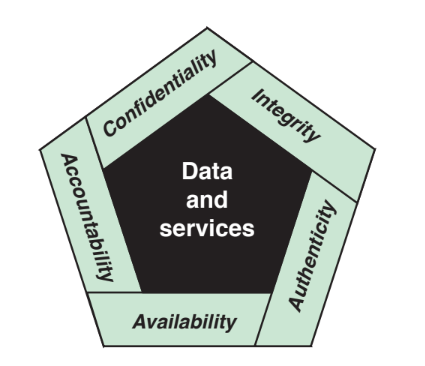
\includegraphics{images/CIA.png}
\end{center}

\newpage
\subsection{Livelli d'impatto}

Analizziamo ora i diversi livelli d'impatto che un attacco può procurare ad una
organizzazione:

\begin{enumerate}
    
    \item \textbf{Impatto basso}, causa una degradazione lieve alle funzioni \\
    dell'organizzazione, che risulta ancora in grado di svolgere le sue funzioni
    principali ma con efficacia ridotta. Può causare danni \textbf{minori} ad
    assets, finanze o danni agli individui;
    \item \textbf{Impatto moderato}, causa una degradazione significativa alle
    funzioni dell'organizzazione, che risulta ancora in grado di svolgere le
    proprie funzioni ma con efficacia nettamente ridotta. Può causare danni
    \textbf{significativi} ad assets e finanze o agli individui, senza includere
    perdite di vite;
    \item \textbf{Impatto elevato}, causa una degradazione severa alle funzioni
    dell'organizzazione, che non risulta più in grado di svolgere una o più
    delle sue funzioni primarie. Può causare danni \textbf{severi o
    catastrofici} ad assets e finanze o agli individui, includendo anche perdite
    di vite. 

\end{enumerate}

\end{document}